\chapter{Badania}

 

%Rozdział przedstawia przeprowadzone badania. Jest to zasadnicza część i~musi wyraźnie dominować w~pracy.
%Badania i analizę wyników należy przeprowadzić, tak jak jest przyjęte w środowisku naukowym (na przykład korzystanie z danych benchmarkowych, walidacja krzyżowa, zapewnienie powtarzalności testów itd). 
%
%\section{Metodyka badań}
%
%\begin{itemize}
%\item opis metodyki badań
%\item opis stanowiska badawczego (opis interfejsu aplikacji badawczych -- w~załączniku)
%\end{itemize}
%
%
%\section{Zbiory danych}
%
%\begin{itemize}
%\item opis danych
%\end{itemize}
%
%
%\section{Wyniki}
%
%\begin{itemize}
%\item prezentacja wyników, opracowanie i poszerzona dyskusja  wyników, wnioski
%\end{itemize}
%
% 
%\begin{table}
%\centering
%\caption{Opis tabeli nad nią.}
%\label{id:tab:wyniki}
%\begin{tabular}{rrrrrrrr}
%\toprule
%	         &                                     \multicolumn{7}{c}{metoda}                                      \\
%	         \cmidrule{2-8}
%	         &         &         &        \multicolumn{3}{c}{alg. 3}        & \multicolumn{2}{c}{alg. 4, $\gamma = 2$} \\
%	         \cmidrule(r){4-6}\cmidrule(r){7-8}
%	$\zeta$ &     alg. 1 &   alg. 2 & $\alpha= 1.5$ & $\alpha= 2$ & $\alpha= 3$ &   $\beta = 0.1$  &   $\beta = -0.1$ \\
%\midrule
%	       0 &  8.3250 & 1.45305 &       7.5791 &    14.8517 &    20.0028 & 1.16396 &                       1.1365 \\
%	       5 &  0.6111 & 2.27126 &       6.9952 &    13.8560 &    18.6064 & 1.18659 &                       1.1630 \\
%	      10 & 11.6126 & 2.69218 &       6.2520 &    12.5202 &    16.8278 & 1.23180 &                       1.2045 \\
%	      15 &  0.5665 & 2.95046 &       5.7753 &    11.4588 &    15.4837 & 1.25131 &                       1.2614 \\
%	      20 & 15.8728 & 3.07225 &       5.3071 &    10.3935 &    13.8738 & 1.25307 &                       1.2217 \\
%	      25 &  0.9791 & 3.19034 &       5.4575 &     9.9533 &    13.0721 & 1.27104 &                       1.2640 \\
%	      30 &  2.0228 & 3.27474 &       5.7461 &     9.7164 &    12.2637 & 1.33404 &                       1.3209 \\
%	      35 & 13.4210 & 3.36086 &       6.6735 &    10.0442 &    12.0270 & 1.35385 &                       1.3059 \\
%	      40 & 13.2226 & 3.36420 &       7.7248 &    10.4495 &    12.0379 & 1.34919 &                       1.2768 \\
%	      45 & 12.8445 & 3.47436 &       8.5539 &    10.8552 &    12.2773 & 1.42303 &                       1.4362 \\
%	      50 & 12.9245 & 3.58228 &       9.2702 &    11.2183 &    12.3990 & 1.40922 &                       1.3724 \\
%\bottomrule
%\end{tabular}
%\end{table}  
%
%\begin{figure}
%\centering
%\begin{tikzpicture}
%\begin{axis}[
%    y tick label style={
%        /pgf/number format/.cd,
%            fixed,   % po zakomentowaniu os rzednych jest indeksowana wykladniczo
%            fixed zerofill, % 1.0 zamiast 1
%            precision=1,
%        /tikz/.cd
%    },
%    x tick label style={
%        /pgf/number format/.cd,
%            fixed,
%            fixed zerofill,
%            precision=2,
%        /tikz/.cd
%    }
%]
%\addplot [domain=0.0:0.1] {rnd};
%\end{axis} 
%\end{tikzpicture}
%\caption{Podpis rysunku po rysunkiem.}
%\label{fig:2}
%\end{figure}
%
%
%\begin{figure}
%\begin{lstlisting}
%if (_nClusters < 1)
%	throw std::string ("unknown number of clusters");
%if (_nIterations < 1 and _epsilon < 0)
%	throw std::string ("You should set a maximal number of iteration or minimal difference -- epsilon.");
%if (_nIterations > 0 and _epsilon > 0)
%	throw std::string ("Both number of iterations and minimal epsilon set -- you should set either number of iterations or minimal epsilon.");
%\end{lstlisting}
%\caption{Przykład pseudokodu}
%\end{figure}


\section{Metodyka badań}

\subsection{Cel badania}

Celem badani jest sprawdzenie wydajności algorytmów wyszukujących na zbiorze
danych dostarczonego w celu wyszukania treści. Dodatkowym celem jest porównanie
działań zaimplementowanego programu z innymi, podobnymi rozwiązaniami.

\subsection{Zakres badania}

Zakres badań obejmuje porównanie prędkości algorytmów w celu ustalenia, który
z nich jest najszybszy pod względem czasu wykonania. Zostanie to ustalone na
mniejszym zbiorze rozpakowanych archiwów. Następnie na nierozpakowanym zbiorze
archiwów porównane zostaną narzędzia pod względem liczby wyszukań oraz prędkości
wyszukań.

\subsection{Hipoteza badań}

Hipotezą badań jest to, że kolejne algorytmy posiadające większe zużycie zasobów
na przygotowanie wyszukania będą wykonywały się szybciej niż te z mniejszym
zużyciem. Hipotezą pomocniczą jest to, iż im większy zbiór informacji zebrany
na podstawie łańcucha szukanego, tym większa prędkość algorytmu. Dodatkową hipotezą jest
to, iż wykorzystanie \english{Garbage Collectora} wpływa na stabilność 
otrzymywanych wyników oraz że czas wykonywania odczytów danych z dysku zajmuje
zdecydowaną ilość czasu.

% \section{Sposób przeprowadzenia badań}
\section{Badanie benchmarku algorytmów}

\begin{figure}[h]
  \centering
  \begin{lstlisting}
go test -test.bench=. -benchmem . -benchtime=1x -count=10

func BenchmarkMorisPrattWindowWord(b *testing.B) {
	var founds = []string{}
	mp := &MorisPratt{}
	filepath.Walk(DIR, WalkAndFindByAlgo(mp,
    &founds, []byte("window")))
	if len(founds) != 11598 {
		b.Fatal("test failed", len(founds), 11598)
	}
}
  \end{lstlisting}
  \caption{Przykład wykonania testu benchmarkowego}
  \label{fig:code:examplePerfTest}
\end{figure}
Badanie zostało przeprowadzone na maszynie autora, podczas działania środowiska
graficznego na Fedora 40. Procesor wykonujący operacje to Intel Core i7-6700K
w architekturze amd64.

Przeprowadzenie badań polegało na uruchomieniu komendy w pierwszej linii (rys. 
\ref{fig:code:examplePerfTest}) i wykonaniu funkcji na algorytmie Morisa Pratta. 
Wykonano 20 testów na wyszukaniu 3 słów, które mogły występować w zbiorze danych,
ze względu na wcześniej przeanalizowaną zawartość. Tymi słowami były 
\textit{"main"}, \textit{"window"}, \textit{"function"}.

\textit{"founds"} jest zmienną przechowującą miejsce znalezionego 
ciągu wyszukiwanego, a zmienna \textbf{mp} to struktura przechowująca implementacje algorytmu MP oraz
Bufor Wcześniejszego Procesowania (BWM) dla ciągu wyszukiwanego. Pierwsza implementacja nie 
posiadała tej struktury i BWM był obliczany przy każdym przebiegu algorytmu.
 To znacznie wpłynęło na prędkość działania algorytmu Boyera-Moora, który posiadał największy BWM.

\begin{Definition}\label{def:WalkFuncGolang}
WalkFunc jest to typ funkcji przyjmowany przez funkcje Walk w module filePath.
Funkcja ta przyjmuje 3 argumenty: ścieżkę, informacje o analizowanym pliku oraz
argument przyjmujący błąd i zwraca błąd. \newline \newline
\textit{type WalkFunc func(path string, info fs.FileInfo, err error) error}
\end{Definition}

W linijce 6 (rys. \ref{fig:code:examplePerfTest}) wykonujemy Przejście (ang. 
\english{Walk}) po drzewie plików w \textit{DIR}, który posiada ścieżkę do 
zbioru danych oraz przyjmuje funkcje zdefiniowaną jako WalkFunc 
\ref{def:WalkFuncGolang}. Z powodu potrzeby czytania tylko zawartości plików,
wykorzystaliśmy funkcje WalkAndFindByAlgo, która będzie czytała pliki, ale 
pozwoli algorytmom podanym w argumencie na przeszukanie zawartości w celu 
znalezienia słowa \textit{"window"}. Po zakończeniu funkcji Walk otrzymano 
tablice znalezionych \textbf{founds}, wypełnioną miejscami, w których wystąpiło 
znalezienie podanego ciągu. W liniach 8-10 każdy test posiada walidacje, aby wszystkie wyniki 
otrzymane przez algorytm, były zgodne z wcześniej ustaloną sumą.

\begin{figure}[h]
  \centering
  \begin{lstlisting}
goos: linux
goarch: amd64
pkg: github.com/gadzbi123/algorytmy/regular
cpu: Intel(R) Core(TM) i7-6700K CPU @ 4.00GHz
BenchmarkMorisPrattFunction-8 1	1041257510 ns/op 264623392 B/op 198976 allocs/op
BenchmarkMorisPrattFunction-8 1	1043653365 ns/op 264645080 B/op 198994 allocs/op
BenchmarkMorisPrattFunction-8 1	1040809273 ns/op 264632096 B/op 198971 allocs/op
BenchmarkMorisPrattFunction-8 1	1043999476 ns/op 264656192 B/op 199008 allocs/op
BenchmarkMorisPrattFunction-8 1	1047795718 ns/op 264641272 B/op 199006 allocs/op
BenchmarkKurtMorisPrattFunction-8 1	1059705156 ns/op 264679568 B/op 199007 allocs/op
BenchmarkKurtMorisPrattFunction-8 1	1044558720 ns/op 264704264 B/op 199016 allocs/op
BenchmarkKurtMorisPrattFunction-8 1	1069466845 ns/op 264722128 B/op 199032 allocs/op
BenchmarkKurtMorisPrattFunction-8 1	1062064344 ns/op 264666880 B/op 199024 allocs/op
BenchmarkKurtMorisPrattFunction-8 1	1062586497 ns/op 264697544 B/op 199018 allocs/op
BenchmarkBoyerMooreFunction-8 1	1163758449 ns/op 264251408 B/op 193795 allocs/op
BenchmarkBoyerMooreFunction-8 1	1142778080 ns/op 264249440 B/op 193831 allocs/op
BenchmarkBoyerMooreFunction-8 1	1127766499 ns/op 264255336 B/op 193817 allocs/op
BenchmarkBoyerMooreFunction-8 1	1169790667 ns/op 264177232 B/op 193775 allocs/op
BenchmarkBoyerMooreFunction-8 1	1128862027 ns/op 264270616 B/op 193811 allocs/op
  \end{lstlisting}
  \caption{Przykładowy rezultat performance}
  \label{fig:perfTestResults}
\end{figure}

W rezultacie wykonania otrzymujemy dane o czasie przebiegu funkcji, ilości 
alokacji oraz ile bajtów wykorzystano na operacje (rys. \ref{fig:perfTestResults}).

\subsection{Zbiór badań}
\begin{table}[h]
    \centering
    \begin{tabular}{|l|l|}
        \hline
        \textbf{Typ MIME} & \textbf{Rozmiar (w KB)}\\
        \hline
application/pdf & 1094989.16  \\
application/zip & 911563.68 \\
application/x-rar & 751425.98 \\
application/gzip & 158709.61  \\
application/postscript & 151226.98 \\
text/html & 49879.89  \\
image/jpeg & 49342.96  \\
image/gif & 42260.80  \\
text/xml & 16914.17  \\
application/x-tar & 10470.00  \\
application/mac-binhex40 & 4704.44 \\
text/plain & 2929.91  \\
application/octet-stream & 2131.61 \\
application/ms.portable-executable & 1552.50  \\
application/x-ms-ne-executable & 1404.35 \\
text/x-c++ & 1139.31\\
application/x-ace-compressed & 1004.49 \\
application/msword & 460.50\\
application/x-compress-ttcomp & 362.78  \\
text/x-c & 332.51  \\
application/x-java-applet & 293.44  \\
application/x-msaccess & 154.00 \\
application/x-dosexec & 117.99 \\
text/x-java & 94.38  \\
application/vnd.ms-cab-compressed & 88.34  \\
text/csv & 54.14  \\
text/x-diff & 46.94 \\
application/wordprocessingml.document & 34.65 \\
text/x-script.python & 1.90 \\
inode/x-empty & 0.00  \\
\hline
Total & 3253691.41  \\
        \hline
    \end{tabular}
    \caption{Ilość danych na podstawie typu MIME}
    \label{tabela:typy-MIME-z-iloscia}
\end{table}
%application/zip                               9312014.35 KB      236
%audio/mpeg                                    2771693.64 KB      541
%application/x-rar                             1358304.96 KB       31
%application/vnd.ms-htmlhelp                    337207.65 KB      100
%application/octet-stream                       302676.00 KB       71
%image/jpeg                                     228285.10 KB     1347
%video/x-ms-asf                                 223755.41 KB       15
%image/vnd.djvu                                 174702.98 KB       24
%application/postscript                          84778.60 KB      442
%application/x-ace-compressed                    83686.03 KB        3
%application/gzip                                72011.68 KB       58
%image/gif                                       38853.47 KB     1622
%text/html                                       38485.94 KB     1788
%application/msword                              29155.00 KB       75
%audio/ogg                                       24242.73 KB       25
%application/x-tar                               20940.00 KB       18
%application/x-dosexec                            9318.01 KB        2
%audio/x-wav                                      9180.17 KB        1
%application/x-bzip2                              6383.85 KB        5
%text/rtf                                         4710.93 KB        2
%application/mac-binhex40                         4704.44 KB        2
%text/x-c++                                       4021.66 KB      347
%video/x-msvideo                                  3731.00 KB        1
%application/vnd.ms-powerpoint                    3420.50 KB        1
%text/x-c                                          987.73 KB      345
%text/plain                                        858.96 KB      136
%text/x-tex                                        748.25 KB       64
%application/winhelp                               216.03 KB        1
%application/pdf                                   112.13 KB        1
%image/x-portable-greymap                           54.24 KB        5
%text/x-diff                                        45.52 KB        2
%application/x-matlab-data                          40.19 KB        1
%message/rfc822                                     31.62 KB        1
%text/xml                                           23.51 KB        1
%application/x-shockwave-flash                      21.97 KB        1
%application/x-ole-storage                          20.00 KB        1
%application/x-winhelp                              16.43 KB        1
%text/x-makefile                                    10.37 KB        7
%image/x-xfig                                        7.15 KB        3
%application/javascript                              6.91 KB        1
%application/x-wine-extension-ini                    2.53 KB        4
%text/x-perl                                         1.92 KB        1
%inode/x-empty                                       0.00 KB       20
%Total                                         15149469.59 KB     7353

Zbiór danych (tab. \ref{tabela:typy-MIME-z-iloscia}) posiadał znaczną ilość 
plików pdf, które w niektórych przypadkach można było odczytać. Gdy pdf został
stworzony z dokumentu tekstowego takiego jak docx czy odt, to zawartość tekstowa
została zawarta w dokumencie pdf. Jeżeli natomiast pdf został stworzony ze skanu
książki, nie zapisała się treść tekstowa. Wtedy cała treść jest przechowana w 
postaci zdjęcia, które nie można odczytać użytym rozwiązaniem.

Możliwość odczytania zawartości daje narzędzie OCR (ang. \english{Optical Character Recognition}).
Narzędzie może służyć do oczytania zawartości plików pdf oraz tekstu z obrazów.
Takie rozwiązanie nie zostanie użyte w pracy, gdyż nie skupiamy się tu na 
algorytmach sztucznej inteligencji.

Pliki audio to piosenki oraz podcasty, których nie można łatwo odczytać algorytmem.
Do oczytania treści z takich plików można wykorzystać narzędzia dokonujące 
trankrypcji, czyli konwertujące rozpoznaną mowę na tekst, jednak te rozwiązania bazują 
na sztucznej inteligencji, które nie są przedmiotem pracy.

Kolejnym problemem okazało się odczytanie plików formatu doc, które są starym 
formatem dokumentów wykorzystywanych przez Microsoft i ich zakodowana treść nie
jest łatwa do odczytu. W odróżnieniu od formatu docx, który jest archiwum, 
narzędzie nie podejmie się odczytania plików doc. Z uwagi na to, że archiwum danych
jest dość stare, nie wystąpiły tam dokumenty formatu docx. Gdyby wystąpił można
by odczytać zawartość archiwów docx w ten sam sposób jak w przypadku innych 
archiwów.

Niestety w przypadku starych plików doc, nie ma możliwości rozpakowania treści
pliku i otrzymania zawartości. Dodatkowo pliki posiadają nietypowe kodowania,
co powoduje dalsze skomplikowanie z odczytania ich treści.

Archiwa posiadają również różne algorytmy kompresji oraz różne sposoby zapisu w zależności od
rozszerzenia np. zip, rar, 7z, tar. To powoduje, że należy wykorzystać wiele
metod konwersji tych plików do faktycznej struktury możliwej do odczytania. 
Biblioteka, którą wykorzystano nie obsługuje plików skompresowanych przez gzip.
To powoduje, że pliki z rozszerzeniem .gz nie będą otwierane.

Pobrane archiwa posiadały brakujące dane i to powodowało, że biblioteka konwertująca
archiwa miała problem z ich otwarciem. Z tego powodu część danych musiała być 
pominięta, aby program nie został przerwany przez SEGV. Wykorzystana biblioteka
musiała zostać niepoprawnie zaimplementowana, gdyż istnieją programy umiejące 
otworzyć te archiwa, choć nie wszystkie z tych narzędzi działały poprawnie.
To wymagało zmniejszenia zbioru przeszukiwanych danych z archiwum i ograniczenia
się do 15 GB danych.

\begin{figure}
\centering
\begin{subfigure}{0.7\textwidth}
    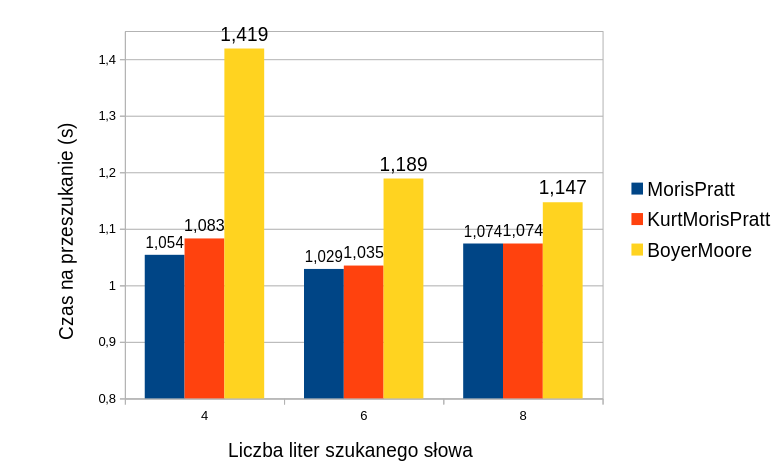
\includegraphics[width=\textwidth]{./images/GraphFirstAttempt.png}
    \caption{Wykres czasów bez statycznego bufora pliku oraz z ponowną 
    rekalkujacją (BWM).}
    \label{fig:GraphFirstAttempt}
\end{subfigure}
%\hfill
\begin{subfigure}{0.7\textwidth}
    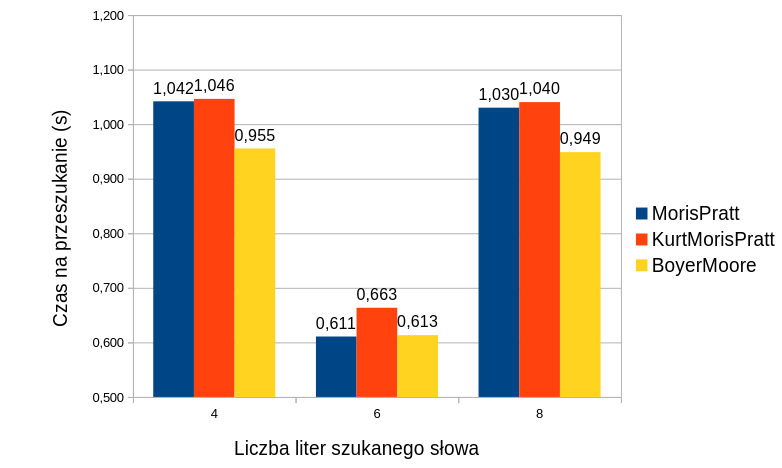
\includegraphics[width=\textwidth]{./images/GraphPreAllocBM.png}
    \caption{Wykres czasów bez statycznego bufora pliku z jednokrotną kalkulacją
     BWM w implementacji algorytmu Boyera-Moore'a. }
    \label{fig:GraphPreAllocBM}
\end{subfigure}
\begin{subfigure}{0.7\textwidth}
    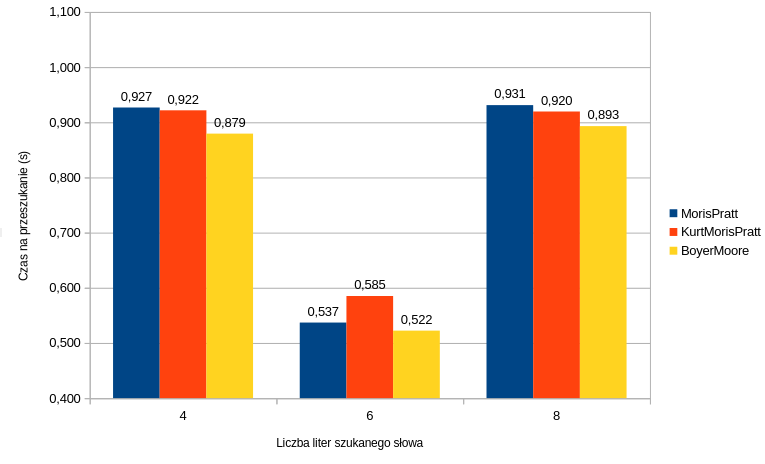
\includegraphics[width=\textwidth]{./images/GraphStaticPreallocAndFileBuffer.png}
    \caption{Wykres czasów ze statycznym buforem pliku oraz jednokrotną kalkulacją BWM dla każdego algorytmu.}
    \label{fig:GraphStaticPreallocAndFileBuffer}
\end{subfigure}
\caption{Wykresy kolejnych iteracji na algorytmach}
\label{fig:GraphsIterationComparison}
\end{figure}

Pierwszy test wydajnościowy, który został przeprowadzony, sprawdzał wszystkie 
foldery, w których znajdowały się pliki. Za drugim razem ograniczono się tylko
do plików, które mogą posiadać oczekiwaną zawartość, odrzucając zatem część 
plików ze zbioru. Wykonano testy na 3 algorytmach, gdzie odczytywano 5191 plików 
i łącznie 240 MB danych. Oto rezultaty określonych algorytmów.

Algorytm Morisa-Pratta jest nieznacznie wolniejszy od algorytmu 
Kurta-Morisa-Pratta. Jest to spowodowane niewielką optymalizacją pomiędzy tymi 
dwoma algorytmami. Według danych na rysunku \ref{fig:GraphFirstAttempt} można 
zauważyć, KMP w niektórych przypadkach jest wolniejszy, niż algorytm MP, 
ponieważ posiada większe odchylenie standardowe, co powoduje, że jest mniej
stabilny. 

%Patrząc na statystki możemy zauważyć, że podczas pracy algorytmów, wystąpiły 
%wartości odstające (ang. \english{Outlier}) w niektórych wykonaniach dla 
%algorytmu KMP. Gdy usuniemy je pojawia się bardziej rzetelna informacja o 
%różnicy pomiędzy wynikami.

Algorytm Boyera-Moore'a wykorzystywany w takich narzędziach jak grep, ma 
wolniejszy czas egzekucji, co wynika z rys. \ref{fig:GraphFirstAttempt}, ale 
algorytm może zostać poprawiony. Z powodu błędnej implementacji, wykonywano
ponowną kalkulację BWM podczas otwarcia nowego pliku, choć szukana fraza pozostawała
taka sama. Wykorzystanie wcześniejszego przeliczonego bufora wpłyneło na znaczne
przyspieszenie algorytmu.

Implementacja, której wyniki widzimy na grafie \ref{fig:GraphFirstAttempt} jest
znacznie wolniejsza od pozostałych algorytmów. Powodem jest spędzanie znacznej
cześć czasu na stworzeniu tablicy wcześniejszego procesowania. Wiadome jest, że zawsze 
sprawdzamy ten sam ciąg we wszystkich plikach w folderze. Istnieje możliwość 
stworzenia tablicy wcześniejszego procesowania przy pierwszym użyciu algorytmu, a następnie
wykorzystanie tej tablicy we wszystkich odczytach.

Na następnym wykresie \ref{fig:GraphPreAllocBM} można zauważyć poprawę, gdy
implementacja algorytmu Boyer-Moora wykorzystuje ten sam bufor wcześniejszego procesowania, a
pozostałe algorytmy tworzą go od nowa, kiedy otwierany jest kolejny plik. Celem 
takiej implementacji było uzyskanie informacji o wpływie ponownego wykorzystania
bufora wcześniejszego procesowania na czas wykonania. 

Aby sprawdzić faktyczne wyniki, należało zaimplementować ponowne wykorzystanie
bufora wcześniejszego procesowania dla wszystkich algorytmów. Wyniki z drugiego wykresu 
potwierdziły wartość ponownego użycia bufora wcześniejszego procesowania w prędkości wykonania
algorytmu.

Ostatni wykres \ref{fig:GraphStaticPreallocAndFileBuffer} przedstawia implementację
wykorzystującą ponownie bufor wcześniejszego procesowania, jak i bufor przechowujący plik.
Bufor wcześniejszego procesowania był przydzielany przy każdym otwarciu nowego pliku,
co powodowało, że ten bufor mógł być zbierane przez \english{Garbage Collector}.
W przypadku użycia stałego bufora zapewniamy, że program nie będzie się pozbywał
bufora, co uniknie proszenia o pamięć systemu. Gdy na początku programu utworzymy
bufor przechowywania pliku sami (nie polegając na optymalizacji języka), algorytm Boyera-Moore'a
odnotował 5 \% poprawę \ref{fig:GraphStaticPreallocAndFileBuffer} w stosunku do poprzedniej implementacji.

Niestety statyczny bufor przechowujący plik, należy alokować, znając rozmiar 
największego pliku w folderze, który wynosił 11 MB. Było tak, gdyż odrzucaliśmy
obrazy. Moglibyśmy przed rozpoczęciem algorytmu sprawdzać rozmiar maksymalny 
pliku, ale to wydłuży czas działania.

Istnieje też sytuacja, w której nie chcielibyśmy największego rozmiaru, ponieważ nie
znamy największego pliku w zbiorze. Podanie zbyt małej ilość na bufor pliku spowoduje,
że nie otrzymamy wszystkich wyników z pliku, gdyż nie zmieści się on w buforze pamięci statycznej.

Można wykorzystać pamięć dynamicznie przydzielaną i w przypadku zbyt małego 
bufora dla danych z pliku, ustawić nowy rozmiar równy zawartości pliku.
Zmniejszy to ilość alokowania nowego bufora, ale nie będzie to aż tak efektywne
w szybkim wyszukiwaniu danych oraz znacząco zwiększy czas działania Garbage Collectora.

W badaniu porównawczym dla programów w następnej sekcji zdecydowano się na
czytanie pojedynczej linii z pliku, który skanujemy. Niestety to podejście
skutkowało takim samym problem jak ten w przypadku bufora pamięci statycznej.

\section{Badanie ilość otrzymanych wyników z programów}

Wybrano kilka narzędzi, które będą porównywane pod względem liczby wyszukiwań
oraz ich prędkości. Narzędzia, które zachowują się podobnie do implementacji
autora do ugrep (ug), zgrep oraz ripgrep (rg). 

\begin{figure}[h]
\centering
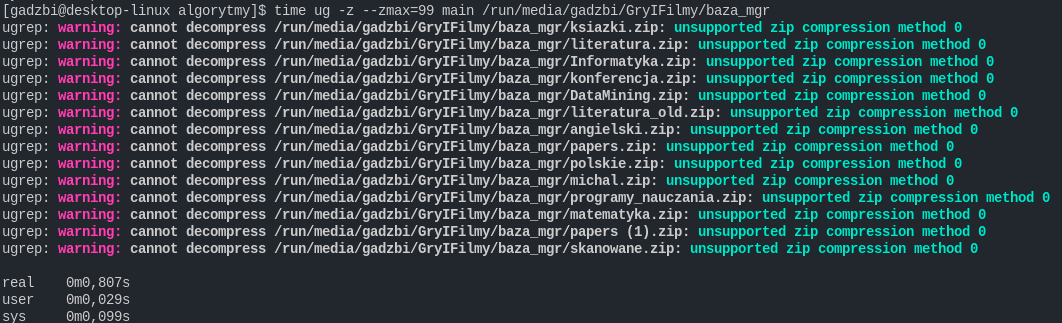
\includegraphics[width=0.7\textwidth]{./images/ugrep-errors.png}
\caption{Niepoprawne działanie programu ugrep dla archiwów pobranych z chmury}
\label{fig:ugrepErrors}
\end{figure}

Wiele z tych narzędzi nie działało poprawnie, gdy próbowaliśmy odczytać zawartość
archiwów. Przykładowo narzędzie ugrep (rys.\ref{fig:ugrepErrors}) nie rozpoznawało 
metody kompresji plików zip, co spowodowało, że nie nie otrzymaliśmy ani 
jednego rezultatu z programu. To powoduje, że narzędzie zostanie wykluczone z 
dalszej analizy.

Możliwym rozwiązaniem byłoby rozpakowanie wszystkich plików innym narzędziem, np.
7z. Następnie wymaga to przeszukanie rozpakowanego pliku oraz rozpakowanie 
zawartego w nim kolejnego archiwum. Po wykonaniu takiego działania można 
odczytać zawartość, co znacznie wydłużyłoby czas działania. Takie podejście również
komplikuje testowanie takiego rozwiązania, bo wykonywane są różne programy, 
które wzajemnie na siebie oczekują. Narzędzie powinno być w stanie samo 
rozpakować i wyszukać wszystkie frazy poszukiwane. Dodatkowo narzędzie powinno
znajdować frazy zaraz po rozpakowaniu pliku i nie powinno czekać na rozpakowanie
wszystkich archiwów, aby przeszukiwać ich zawartość.

\begin{figure}[h]
\centering
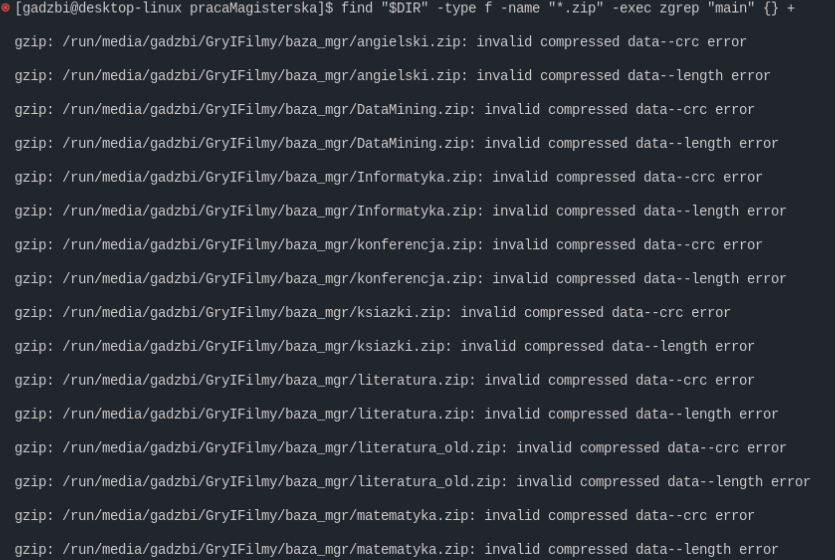
\includegraphics[width=0.7\textwidth]{./images/zgrep-errors.png}
\caption{Niepoprawne działanie programu zgrep z pomocą finda}
\label{fig:zgrepErrors}
\end{figure}

Kolejne z wymienionych narzędzi również nie spełnia wymagań. Zgrep nie pozwala
na rekurencyjne wyszukiwanie danych w folderach, w których znajdują się archiwa.
Nawet zastosowanie pomocniczego narzędzia find w celu wykonania zadania,
powoduje, że program nie jest w stanie przeskanować archiwów (rys. \ref{fig:zgrepErrors}).

Otrzymany błąd sugeruje, że długość danych w archiwum nie jest zgodna. Dodatkowo
mamy informacje o błędzie w wartości cyklicznej kontroli nadmiarowej CRC
(ang. \english{Cyclic Redundancy Check}). Ta wartość to system sum kontrolnych
pozwalający na wykrycie błędów zmagazynowanych danych. Zgrep nie pozwala 
rozpakować i przeszukać zawartości szukanych archiwów.

\begin{figure}[h]
\centering
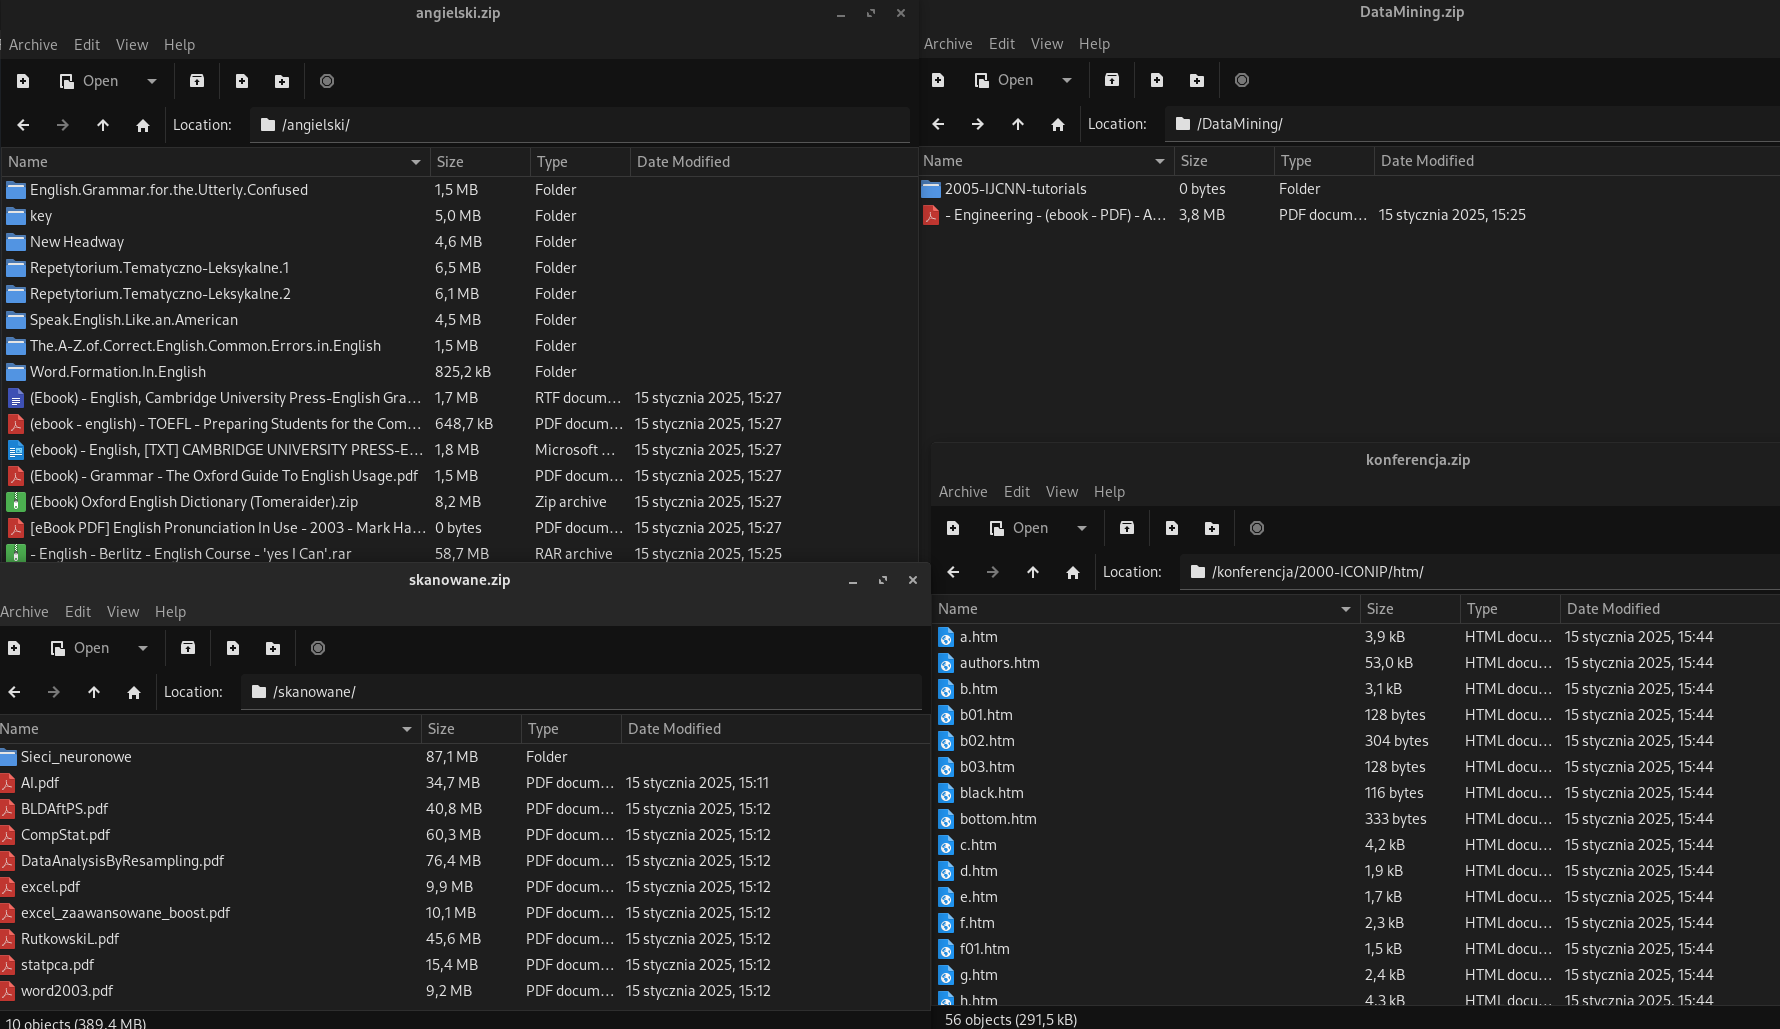
\includegraphics[width=0.7\textwidth]{./images/przykład-otwarcia-archiwów.png}
\caption{Przykład otwarcia archiwów przez program graficzny Engrampa}
\label{fig:engrampaExample}
\end{figure}

Archiwa jednak są możliwe do otworzenia przez program graficzny Engrampa \cite{bib:internet:EngrampaArchives}.
Choć wszystkie pliki zostały odczytane, oznacza to, że istnieje możliwość pozyskania
części zawartości (rys. \ref{fig:engrampaExample}).

Narzędzie graficzne nie będzie brane pod uwagę do badania, zostało jedynie podane
jako przykład poprawności archiwów.

\begin{figure}[h]
\centering
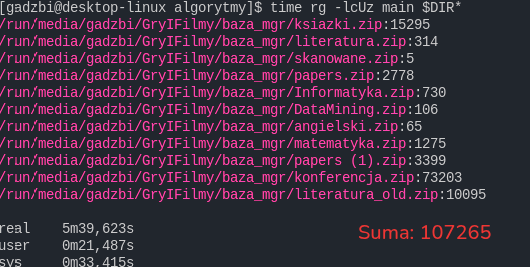
\includegraphics[width=0.7\textwidth]{./images/ripgrep-result-main.png}
\caption{Przykładowy rezultat wykonania komendy ripgrep ze zmierzonym czasem}
\label{fig:ripgrepResultMain}
\end{figure}

Narzędzie ripgrep pozwala na wyszukanie zawartości w archiwach i działa bardzo dobrze.
Narzędzie było w stanie wyszukać ogromną liczbę fraz "main" we wszystkich plikach \ref{fig:ripgrepResultMain}.
Narzędzie niestety nie posiada dokładnej lokalizacji, w której wystąpiło wyszukanie,
tylko jest w stanie wskazać miejsce w pliku skompresowanym konkretny bajt.
Taki rezultat nie mówi, w którym pliku znajdują się frazy, a jedynie może znaleźć 
kontekst w pliku lub podać ilość wystąpień.

Różnica ta jest znacząca w celu znalezienia frazy w konkretnym pliku. 
Implementacja gsearch pozwala na wyszukanie linii pliki, w którym fraza się znajduje. 

\begin{figure}[h]
\centering
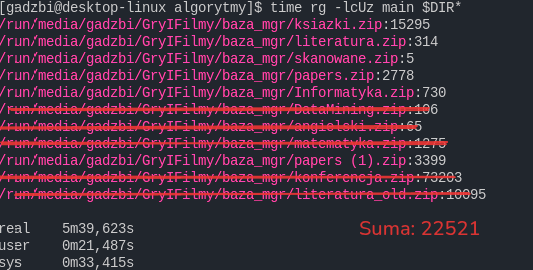
\includegraphics[width=0.7\textwidth]{./images/rgSkippedmain.png}
\caption{Liczba wystąpień "main" z pominięciem kilku archiwów}
\label{fig:ripgrepRemoveSkipped}
\end{figure}

Autorskim programem do przeszukiwania treści w archiwach jest gsearch. Od teraz
wszystkie odniesienia do implementacji będą odnosiły się do nazwy programu.

Gdy gsearch próbuje przeszukać archiwum z niepoprawną sumą kontrolną, program
zostaje wyłączony z powodu błędu. Gsearch może wykonać pełne szukanie w przypadku,
gdy suma kontrola plików archiwów jest poprawna.

Gdy gsearch przeszukuje archiwa nieuszkodzone \ref{fig:ripgrepRemoveSkipped},
to widać, że liczba wystąpień w gsearch jest większa. Poniżej znajduje się zestawienie
ilości znalezionych wystąpień dla wszystkich archiwów przeszukiwanych przez rg,
pominiętych archiwów dla rg oraz pominiętych archiwów przeszukanych przez gsearch.

Należy wspomnieć, iż jedno wystąpienie dla ripgrepa to pojawienie się frazy
w danej linijce. W ten sam sposób liczone jest znalezienie wystąpienia w gsearch.
Implementacja gsearch nie posiada wrażliwości na wielkość liter, dlatego nie 
jest testowana.

\begin{table}[h]
    \centering
    \begin{tabular}{|r|r|r|r|}
        \hline
        \textbf{Fraza (litery)} & \textbf{rg (wszystkie archiwa)} & \textbf{rg (pominięte)} &  \textbf{gsearch (pominięte)} \\
        \hline
        wan (3) & 34821 & 22951 & 20293 \\
        \hline
        main (4) & 107265 & 22521 & 23822 \\
        \hline
        window (6) & 16998 & 8251 & 9430 \\
        \hline
        analysis (8) & 3511 & 2168 & 1740 \\
        \hline
        book desc (9) & 6 & 3 & 3 \\
        \hline
        informatyka (11) & 1 & 1 & 5 \\
        \hline
        wInDoW (6) & 56760 & 20939 & 0 \\
        \hline
    \end{tabular}
    \caption{Tabela zestawienia wyników wyszukiwania dla działających programów}
    \label{tabela:iloscWyszukanDziekiProgramom}
\end{table}

Tabela \ref{tabela:iloscWyszukanDziekiProgramom} przedstawia wyniki ilości 
wystąpień fraz w zbiorze archiwów. Ponieważ implementacja gsearch nie potrafi
przeszukać określonych archiwów, zdecydowano się na zestawienie rezultatów
ripgrepa ze wszystkich archiwów, oraz z tego samego zbioru archiwów pominiętych. 

\begin{figure}[ht]
    \centering
    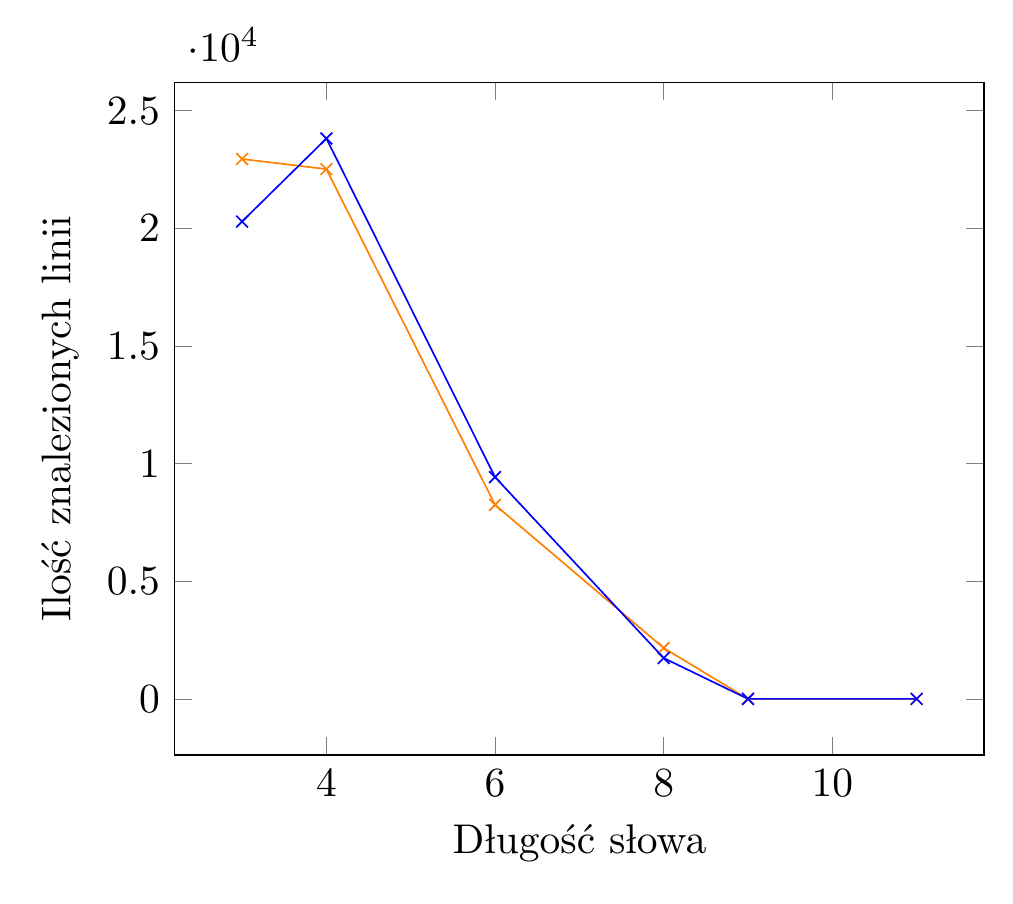
\begin{tikzpicture}[scale=1.50]
        \begin{axis}[
        xlabel=Długość słowa,
        ylabel=Ilość znalezionych linii]
        \addplot[color=orange,mark=x]coordinates{
            (3,22951)
            (4,22521)
            (6,8251)
            (8,2168)
            (9,3)
            (11,3)
        };
        \addplot[color=blue,mark=x]coordinates{
            (3,20293)
            (4,23822)
            (6,9430)
            (8,1740)
            (9,3)
            (11,5)
        };
        \end{axis}
    \end{tikzpicture}
    \caption{Wykres wystąpień linii z frazami w zależności od długości liter w słowie }
    \label{fig:wykresPorównaniaIlosciWystapień}
\end{figure}

Ostatni wiersz pokazuje jakie znaczenie ma wyszukiwanie po wielkości liter 
(tab. \ref{tabela:iloscWyszukanDziekiProgramom}). Program ripgrep posiada 
możliwość ignorowania wielkości liter czego nie robi program gsearch. Jeżeli
nie znamy dokładnej wielkości liter frazy, to może to spowodować brak 
znalezienia frazy (rys. \ref{fig:wykresPorównaniaIlosciWystapień}). 

Program ripgrep nie jest w stanie znaleźć zawartości archiwów zagnieżdżonych w
innych archiwach. Rozwiązuje ten problem gsearch i pozwala na wyszukanie 
znalezienie konkretnego pliku w którym fraza się znajduje.

\section{Porównanie prędkości wyszukiwania programów}

Porównane zostaną programy, które pozwoliły uzyskać oczekiwany rezultat i są to
ripgrep oraz implementowany gsearch. 
Porównanie szybkości wyszukiwania zostanie wykonane na pomniejszonym zbiorze,
aby porównanie czasów było sprawdzane na tym samym zbiorze, gdzie oba programy
są w stanie odczytać z nich dane.

\begin{figure}[ht]
    \centering
    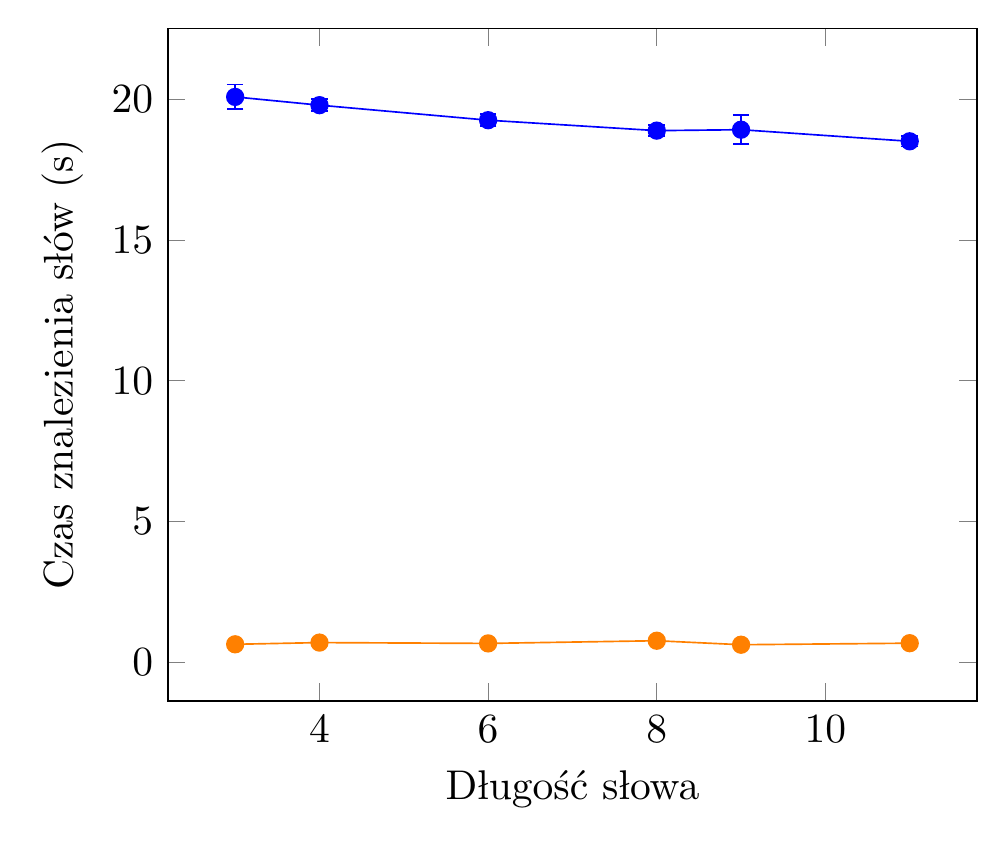
\begin{tikzpicture}[scale=1.50]
        \begin{axis}[
        xlabel=Długość słowa,
        ylabel=Czas znalezienia słów (s)]
        \addplot[color=orange,mark=*,error bars/.cd, y dir=both, y explicit]coordinates{
(3,0.6393700976599999)+=(0,0.007651709374308371)-=(0,0.007651709374308371)
(4,0.69975840454)+-(0,0.02174176683244841)
(6,0.6708412953200001)+-(0,0.04320545697230668)
(8,0.76563712796)+-(0,0.041486089097604)
(9,0.62396489284)+-(0,0.007851351947769116)
(11,0.6782059222)+-(0,0.04570502275958309)
        };
        \addplot[color=blue,mark=*,error bars/.cd, y dir=both, y explicit]coordinates{
(3,20.081044353359996)+-(0,0.4395975771554202)
(4,19.78817344134)+-(0,0.20913605765611032)
(6,19.25416691472)+-(0,0.21635912584660782)
(8,18.88328445046)+-(0,0.19096399774593745)
(9,18.916769088339997)+-(0,0.5162741966007814)
(11,18.5046544439)+-(0,0.17920383136563042)
        };
        \end{axis}
    \end{tikzpicture}
    \caption{Wykres czasów znalezienia fraz w zależności od długości liter dwóch programach}
    \label{fig:wykresPorównaniaCzasówWyszukań}
\end{figure}

Prędkości wyszukiwania danych za pomocą ripgrepa są znacznie większe niż te
za pomocą gsearch (rys. \ref{fig:wykresPorównaniaCzasówWyszukań}). Wynika to z
tego, że ripgrep wykonuje wyszukiwania z wykorzystaniem kilku wątków. Dodatkowo 
program rg ładuje pliki prosto do pamięci, natomiast program gsearch rozpakowuje
zawartość pliku archiwum do folderu, a następnie czyta zawartość każdego pliku.

Takie podejście było konieczne, gdyż Golang ma wbudowane większe ograniczenia w 
proces alokowania danych i tego ile danych może przechowywać w pamięci w danym momencie.

Wykorzystanie innego języka dającego większą swobodę w manipulowaniu pamięcią 
dałoby lepsze czasy wykonania, jednak wykorzystanie języka niskopoziomowego,
wiąże się z większym czasem implementacji algorytmów oraz trudniejszym procesem
analizowania błędów.

Ripgrep dla fraz o długości 3 lub mniejszych używa algorytmu Teddy. Ten algorytm
pozwala na załadowanie całej frazy do rejestru XMM i wykonania bitowego 
porównania małej frazy z zawartością danych przeszukiwanych.

\section{Ripgrep, a pamięć tymczasowa}


\begin{figure}[h]
    \centering
    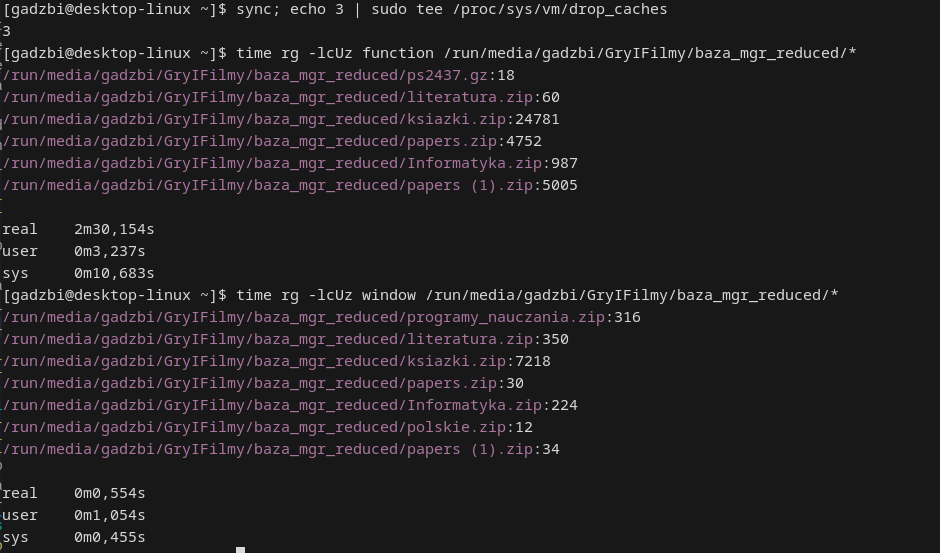
\includegraphics[width=0.7\textwidth]{./images/ripgrep-clear-cache-slow.png}
    \caption{Ripgrep działa wolniej bez pamięci tymczasowej}
    \label{fig:ClearCacheRipgrep}
\end{figure}

Ripgrep posiada bardzo nietypowe działanie w przypadku kolejnych wykonań 
programu. Po pierwszym wykonaniu programu dane z dysku są znacznie dłużej
wyszukiwane. Pomimo że program nie wykorzystuje operacji zachowania danych
w pamięci tymczasowej (cache), to wykorzystuje jakiś mechanizm zapisu 
poprzedniego rezultatu. Gdy wyczyścimy cache jak na obrazie \ref{fig:ClearCacheRipgrep},
zauważamy znaczną pogorszenie rezultatów. Pierwsza komenda zapewnie brak utraty
danych, a następnie druga komenda powoduje zapisanie pliku drop caches z wartością 3.
Ta komenda czyści wszystkie zapisane zawartości pliku oraz dane o odczytywanych
folderach i plikach.

\begin{figure}[ht]
    \centering
    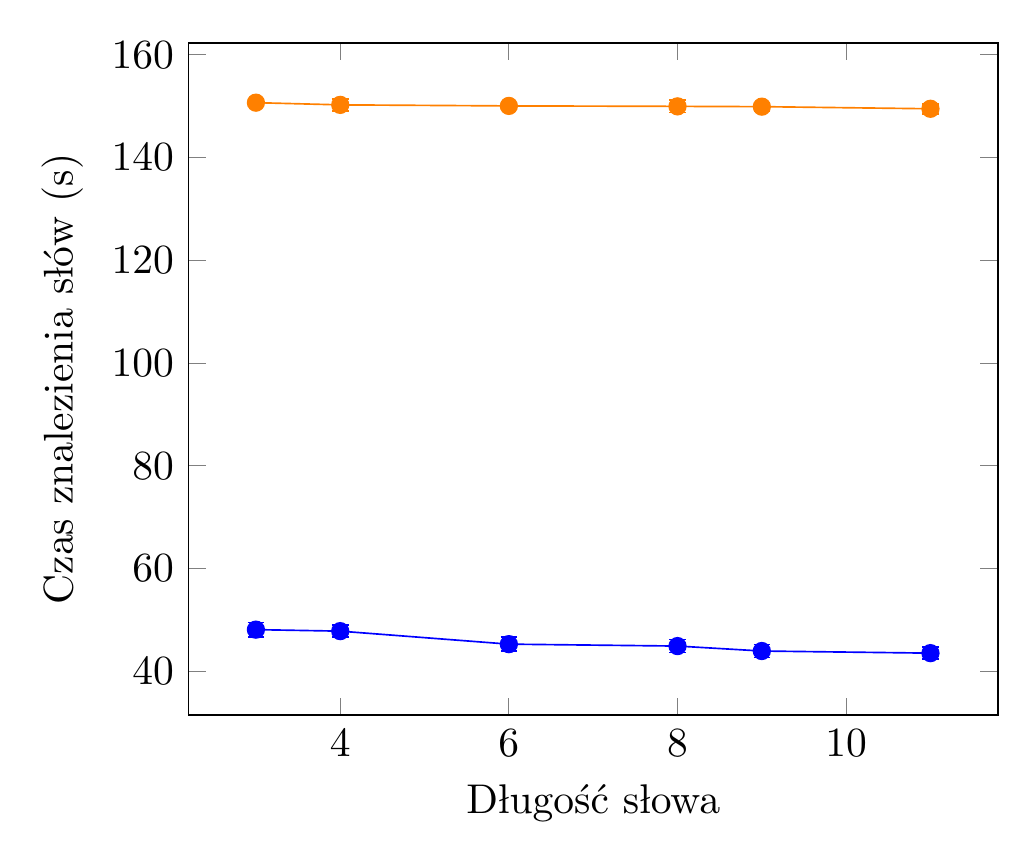
\begin{tikzpicture}[scale=1.50]
        \begin{axis}[
        xlabel=Długość słowa,
        ylabel=Czas znalezienia słów (s)]
        \addplot[color=orange,mark=*,error bars/.cd, y dir=both, y explicit]coordinates{
(3,150.6928509870)+-(0,0.5395975771554202)
(4,150.2652969279)+-(0,1.1823469234769377030)
(6,150.0637899279)+-(0,0.6528969286296298698)
(8,149.9745325373738)+-(0,1.189532878378378387)
(9,149.916769088339997)+-(0,0.842131516816698)
(11,149.5046544439)+-(0,0.9863929239459696)
        };
        \addplot[color=blue,mark=*,error bars/.cd, y dir=both, y explicit]coordinates{
(3,48.081044353359996)+-(0,1.374358456463532)
(4,47.78817344134)+-(0,1.152637838)
(6,45.25416691472)+-(0,1.3674374846352352)
(8,44.88328445046)+-(0,1.26889999)
(9,43.916769088339997)+-(0,1.26626327888)
(11,43.5046544439)+-(0,1.17920383136563042)
        };
        \end{axis}
    \end{tikzpicture}
    \caption{Wykres czasów znalezienia fraz po wyczyszczeniu pamięci tymczasowej}
    \label{fig:wykresPorównaniaCzasówWyszukańUncached}
\end{figure}

Ta komenda powoduje spowolnienie działania obu programów, jednak w znacznie
mniejszym stopniu w przypadku gsearch niż ripgrep \ref{fig:wykresPorównaniaCzasówWyszukańUncached}.
Można również zauważyć większy nierówność czasów wyszukiwań, natomiast
ogólny czas działania programu jest o połowę krótszy niż w przypadku ripgrep.

\section{Wykorzystanie profilowania do oczytania charakterystyki programu}

\begin{figure}[h]
  \centering
  \begin{lstlisting}
f, _ := os.Create("profile.pprof")
pprof.StartCPUProfile(f)
defer pprof.StopCPUProfile()
  \end{lstlisting}
  \caption{Dodanie profilowania do programu gsearch}
  \label{fig:code:profilerGsearch}
\end{figure}

Można również sprawdzić charakterystykę programu gsearch dodając kod na początek 
wykonania programu (rys. \ref{fig:code:profilerGsearch}). Wykonanie programu na
słowie "informatyka" utworzy plik profile.pprof. Ten plik można przejrzeć w 
przeglądarce wcześniej wykorzystując komendę \textbf{go tool pprof -http=localhost:8090 profile.pprof}.

\begin{figure}[h]
\centering
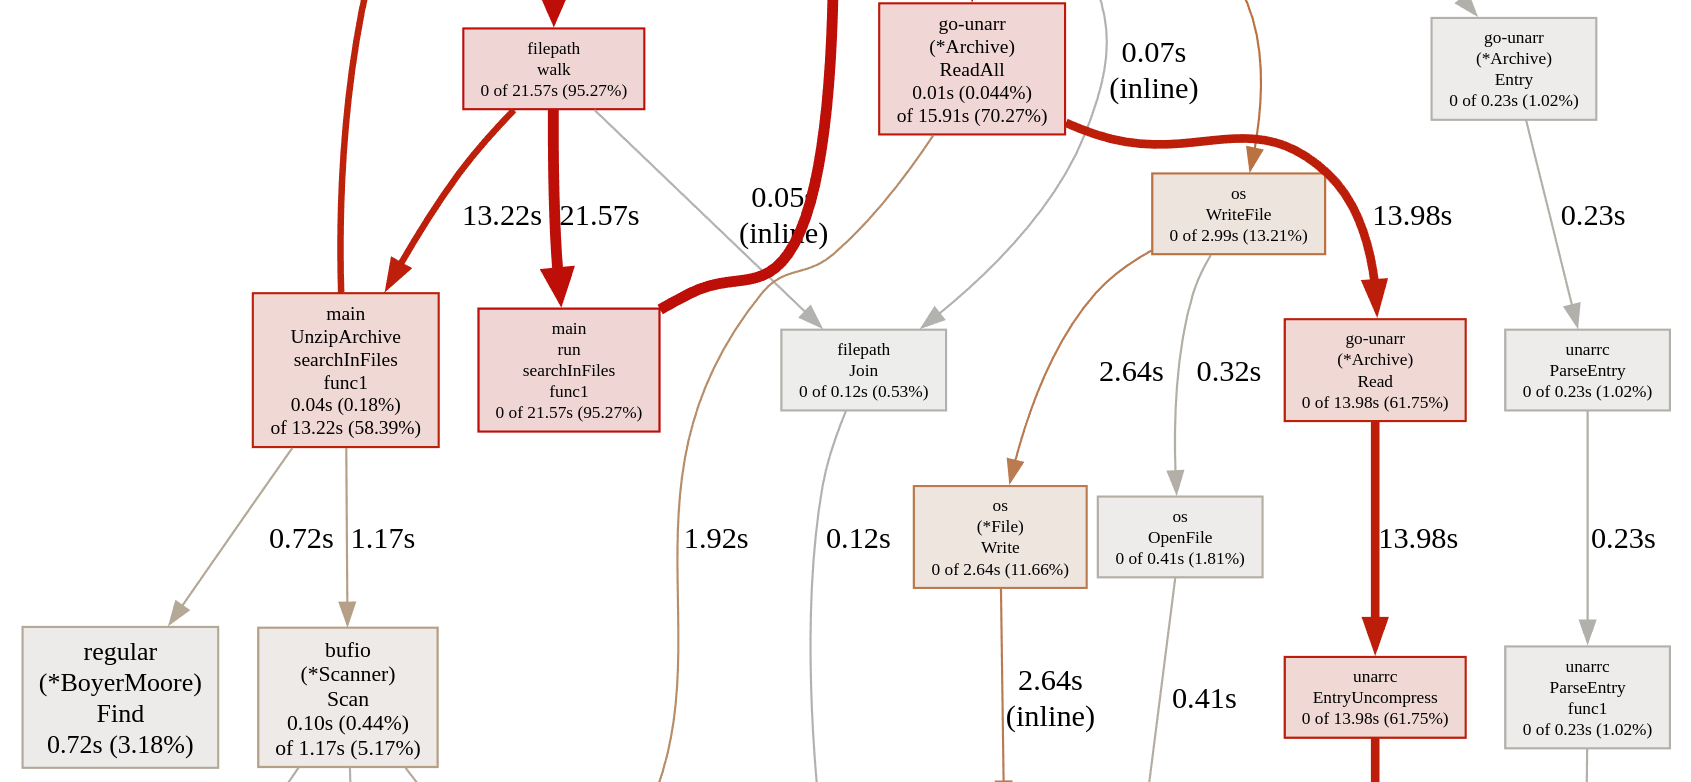
\includegraphics[width=0.7\textwidth]{./images/profiler1.png}
\caption{Przykład grafu wykonań funkcji w gsearch}
\label{fig:profilerGsearch1}
\end{figure}

Po wykonaniu komendy w przeglądarce otworzy się widok na graf programu (rys. \ref{fig:profilerGsearch1}).
Graf jest bardzo skomplikowany do analizy w przypadku, gdy program wykorzystuje rekursje do
przeszukiwania folderów i rozpakowywania zawartości.

Można zauważyć, że większość czasu programu wykorzystywana jest na operacje 
ekstrakcji archiwów i czytania archiwów. Sam algorytm przeszukujący (dolny lewy 
róg rys. \ref{fig:profilerGsearch1}) wykonuje się jedynie 0.72 sekundy.

\begin{figure}[h]
\centering
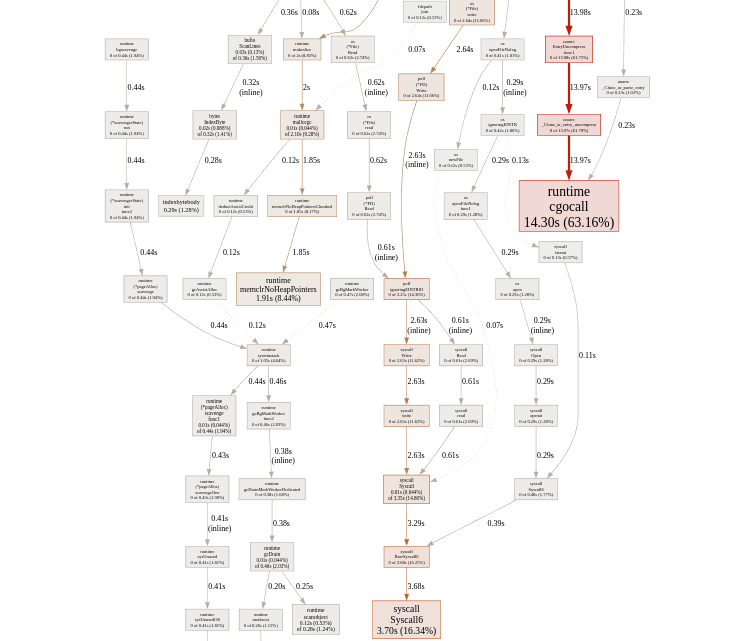
\includegraphics[width=0.7\textwidth]{./images/profiler2.png}
\caption{Zdjęcie grafu funkcji "runtime cgocall" oraz "syscall6"}
\label{fig:profilerGsearch2}
\end{figure}

Głównym ograniczeniem prędkości działania jest czas odczytywania zawartości z plików.
Funkcje "runtime cgocall" oraz "syscall6" stanowią znaczną część czasu
wykonywania programu (rys. \ref{fig:profilerGsearch2}), które wykonują operacje
odczytu zawartości treści z dysku.